\Chapter{Az elkészített alkalmazások áttekintése}

\Section{Demó programok}

Az egyes funkciók fejlesztéséhez és teszteléséhez külön kisebb programok készültek.
Ezek külön csomagokba kerültek.
A következőkben a futtatható modul nevét követően találhatjuk ezeknek a kisebb alkalmazásoknak a célját, a használatuk és működésük főbb jellemzőit.

\bigskip

\noindent \texttt{aruco\_test.test\_aruco}

\medskip

Az \textit{ArUco} marker detektálását lehet vele tesztelni.
Az \texttt{images} mappában található 12 képen lévő markert próbálja felismerni.
Amennyiben sikerült, akkor kirajzolja a marker koordinátarendszerének origójához tartozó triédert, és visszaadja annak eltolását és elforgatását a kamerához képest (\texttt{rvec} és \texttt{tvec}) vektorok.
Ezek, mint eredmények a \texttt{results} jegyzékbe kerülnek.

\bigskip

\noindent \texttt{camera\_background\_with\_obj.camera\_cap\_with\_obj}

\medskip

A program azt mutatja be, hogy a kameraképet hogyan lehet a háttér textúrájaként használni.
Erre rajzol még egy további objektumot.
Az objektum és a textúra betöltése ebben az esetben is az \texttt{objloader} modul segítségével történik.
A pingvin modellje a \texttt{models} mappában található.
A programból a \texttt{q} billentyű megnyomásával lehet.

\bigskip

\noindent \texttt{camera\_calibration.calibration}

\medskip

A kamera kalibrációját mutatja be egy sakktábla mintázat és az \textit{OpenCV} szabványos eszközei használatával.
A kalibrációhoz felhasznált képek az \textit{images} mappában találhatók.
A kalibráció eredményét a \texttt{log.json} állományba menti ki egy kamera mátrix és disztorziós együtthatók formájában \cite{opencvcalib}.
(A harmadik fejezetben említett kamera kalibrálás erre a demó programra épül.) 

\bigskip

\noindent \texttt{camera\_calibration\_and\_aruco\_demo.calibration}

\medskip

A kamera kalibrálását követően az \textit{ArUco} marker követését mutatja be \cite{arucotracking}.

\bigskip

\noindent \texttt{camera\_func.camera}

\medskip

Az aktuális kameraképet visszaadó függvény szerepel benne.
	
\bigskip

\noindent \texttt{camera\_texture\_on\_a\_cube.cam\_cap\_texture\_on\_cube}

\medskip

A kamera képből készült textúra kerül egy kirajzolt kockára.

\bigskip

\noindent \texttt{draw\_cube.draw\_cube}

\medskip

Egy színes oldalapokkal rendelkező kocka rajzolódik ki egy \textit{GLUT} ablakba.
	
\bigskip

\noindent \texttt{draw\_scene.draw\_scene}

\medskip
	
A játék egy lehetséges kezdő állását bemutató rövid programkód.

\bigskip

\noindent \texttt{draw\_texture\_from\_camera.camera\_cap\_texture}

\medskip

A kameraképet, mint textúrát használja egy \textit{GLUT} ablak háttereként.

\bigskip

\noindent \texttt{draw\_trieder.draw\_trieder}

\medskip

Az origóhoz tartozó triéder megjelenítését mutatja be.

\bigskip

\noindent \texttt{game.game}

\medskip

Az elkészült kollaboratív teret megvalósító program egy korábbi, egyszerűbb verziója.
Nem használ \textit{ArCco} marker felismerést, és nincs benne szerver-kliens kommunikáció.
Ilyen formában egy egyszerű \textit{OpenGL} játéknak tekinthető, amiben ugyan az a feladat, mint az elkészült, teljes változatban.
Ebben még minden kút aktív és nincs korlátozás az egymás után következő egy színű dobozok eltűntetésével kapcsolatban.
Az egyik pingvin a \texttt{w,s,a,d,e,space} a másik a \texttt{i,k,l,j,o,p} billentyűkkel irányítható.
	
\bigskip

\noindent \texttt{game\_with\_aruco.game}

\medskip
	
Szintén a kollaborációs tér egy előzetes változata.
Itt már megtörténik a marker felismerése és az arra való rajzolás, azonban ez sem többfelhasználós.
A szabályok ugyanazok, mint a teljes változatban, és az irányítás is megegyezik azzal.

\bigskip

\noindent \texttt{keyboard.keyboard}

\medskip
	
A koordinátarendszer origójába kirajzol egy triédert.
A nyíl billyentyűkkel előre, hátra illeve két oldalra lehet mozogni a kamerával.
A szóköz billentyű megnyomása után felfelé mozdul el a kamera.

\bigskip

\noindent \texttt{keyboard\_with\_cube.keyboard\_cube}

\medskip

Egy kocka objektum mozgatását mutatja be a program, amelyben még a triéder is megjelenítésre kerül.
	
\bigskip

\noindent \texttt{keyboard\_with\_obj.keyboard\_obj}

\medskip
	
Szintén egy objektum mozgatását mutatja be a program, de már egy OBJ fájlból betöltött textúrázott modellen keresztül.

\bigskip

\noindent \texttt{load\_grab\_animation.grab}

\medskip
	
Betöltődnek a \texttt{models} mappában található pingvin modellek és kirajzolódnak váltva egymás után. A fázisok között meg van adva kis késeltetés.
Ez az animáció mutatja be a doboz tolásánál a kéz emelését.

\bigskip

\noindent \texttt{load\_jump\_animation.jump}

\medskip

A pingvin karakter ugrás animációját mutatja be a program.

\bigskip

\noindent \texttt{load\_obj.load\_obj.py}

\medskip

A textúrázott objektum betöltését és megjelenítését mutatja be a program.

\bigskip

\noindent \texttt{load\_release\_animation.release}

\medskip

Az animáció a doboz tolása utána a doboz elengedését mutatja be.

\bigskip

\noindent \texttt{load\_walk\_animation.walk}

\medskip

A séta animációját jeleníti meg a program.

\bigskip

\noindent \texttt{makeGlutWindow.glutwindow}

\medskip

A \textit{GLUT} ablak inicializálására és a \texttt{glutMainLoop} használatára egy példa.

\bigskip

\noindent \texttt{simple\_camera.camera}

\medskip

A kamera kép lekérdezését és megjelenítését mutatja be a program.

\bigskip

\noindent \texttt{trackAruco.trackAruco}

\medskip

A kamera kalibrációja során megkapott mátrixot és együtthatókat betöltve és
felhasználva mutatja a program a marker detektálását egy kapott képen.
Amennyiben talál markert, vissza adja a marker eltolását és elforgatását a kamerához képest.

\bigskip

\noindent \texttt{trackAruco\_and\_draw\_Castle.track\_and\_draw}

\medskip

Az \textit{ArUco} marker felismerését majd egy kastély modell rajzolását mutatja be a program.

\bigskip

\noindent \texttt{trackAruco\_and\_draw\_Cube.track\_and\_draw}

\medskip
	
Az \textit{ArUco} marker felismerését majd arra egy kocka rajzolását mutatja be a program.

\bigskip

\noindent \texttt{trackAruco\_and\_draw\_model.track\_and\_draw}

\medskip
	
Az előző programhoz hasonlóan a marker detektálást mutatja be, de már egy textúrázott modellel.

% \url{https://stackoverflow.com/questions/50764623/object-is-wrong-displaced-in-ar-aruco-opengl}


\Section{A kollaborációs környezetet megvalósító program}

Az előzőekben felsorolt demó alkalmazások azért voltak szükségesek, hogy a dolgozat eredeti céljaként szereplő, kollaboratív feladat megoldását segítő alkalmazást azok alapján fel lehessen építeni.
Az alkalmazás helyes működéséhez szükség van egy \textit{ArUco} markerre, mint amilyen \aref{fig:marker}. ábrán látható.

Felhasználható marker: 
\begin{figure}[htp]
	\centering
	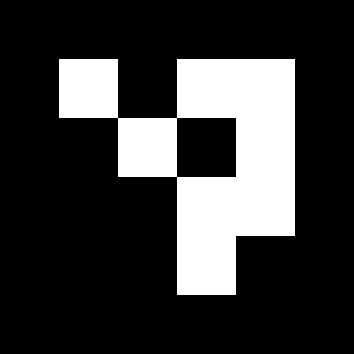
\includegraphics[scale=0.5]{images/marker.png}
	\caption{marker (forrás: \url{https://chev.me/arucogen/})}
	\label{fig:marker}
\end{figure}

Az alkalmazás célja, működése, elkészítésének menete a korábbi fejezetekben már részletezésre került, ezért itt már elegendő csak az implementáció egyes sajátságaira kitérni.

\Aref{fig:game}. ábrán láthatunk a programról egy képernyőképet.

\begin{figure}[htp]
	\centering
	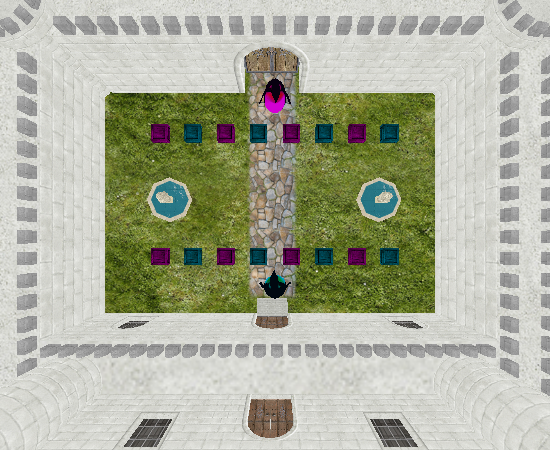
\includegraphics[scale=0.7]{images/game.png}
	\caption{Egy felülnézetes kép a programról}
	\label{fig:game}
\end{figure}

Nyilvánvalóan a program sajátságát az adja, hogy ez a térrész egy, fizikailag létező viszonyítási pontként tekintett marker körül jelenik meg.
A programról, az eszközök elrendezéséről és ezek környezetéről láthatunk egy képet \aref{fig:real}. ábrán.

\begin{figure}[h!]
	\centering
	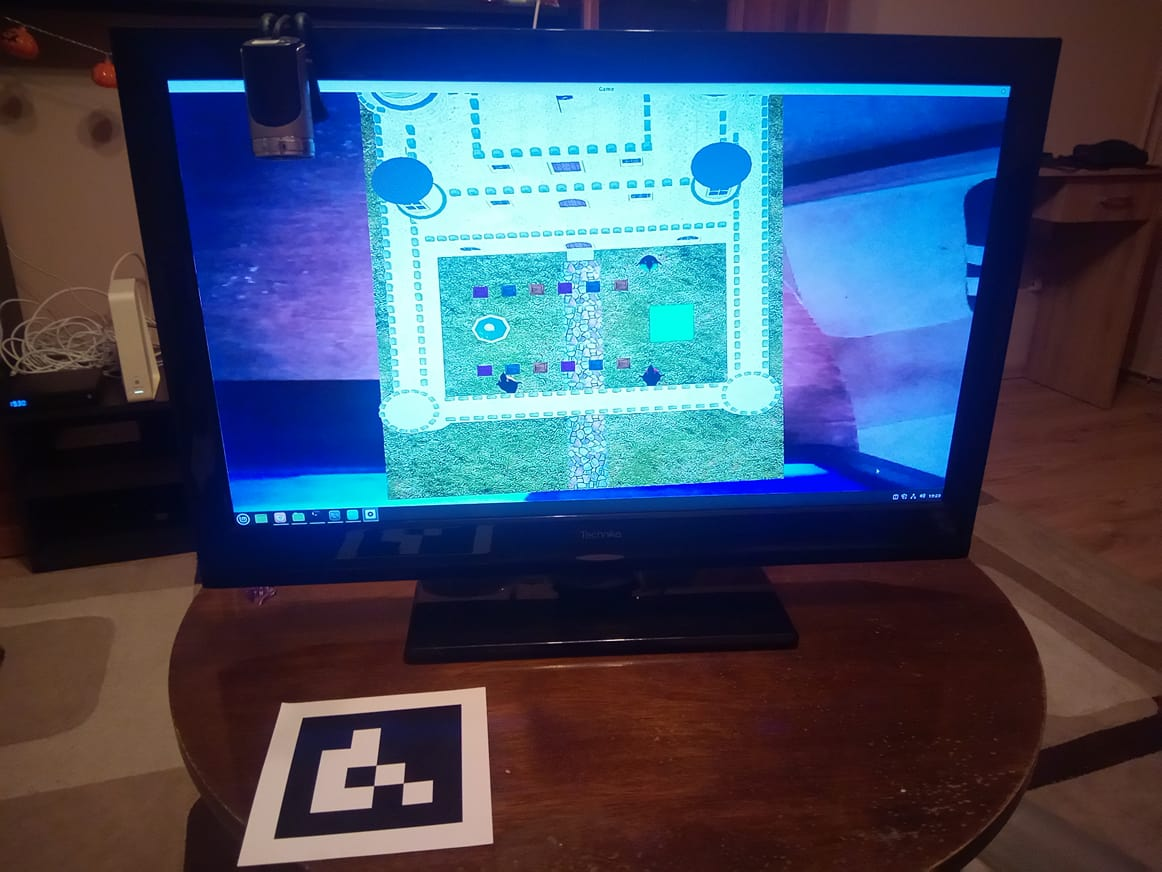
\includegraphics[width=\textwidth]{images/real.jpg}
	\caption{A program és környezete}
	\label{fig:real}
\end{figure}

Érdemes megnézni, hogy a kastély modellje az asztal képére kerül rá a rendereléskor.
A kastélyról így nyilván egy közel felülnézeti kép készül.
Az is látható, hogy a virtuális térben aktuálisan három résztvevő van.

Az alkalmazás működéséhez szükséges futnia a \texttt{server.py} szkriptnek.
Ez az 5000-es porton hoz létre egy lokális szervert, amelyhez aztán csatlakozni fognak tudni a kliensek.

A kliens alkalmazás a \texttt{game.py} szkripttel indítható.
Ez indításkor lekérdezi a szervertől a saját azonosítóját.
Ez alapján dől el, hogy melyik lesz az irányítható karakter a kliens számára.

A virtuális térben való kooperáció akkor igazán szemléletes, hogy ha a résztvevők fizikálisan egy térben vannak, és ugyanazon markert követik az eszközeikkel.
Ekkor ugyanis valóban a valóság egy virtuálisan kiterjesztett része lesz a program által létrehozott kollaborációs környezet.
